%\documentclass[handout]{beamer}
\documentclass{beamer}

\usepackage{beamerthemesplit}
\usepackage{shadowtext}
\usepackage{color}
\usepackage{xcolor}
\usepackage[utf8]{inputenc}

 \usetheme[]{Madrid}
%\usetheme[]{Copenhagen}
%\usetheme{Warsaw}

% El que uso habitualmente:
%\usetheme[height=0.7cm]{Rochester}

% A dark look
%\usecolortheme{beetle}
% A light look:
 \usecolortheme{dolphin}
 
\setbeamertemplate{footline}
{
  \leavevmode%
  \hbox{%
  \begin{beamercolorbox}[wd=.5\paperwidth,ht=2.25ex,dp=1ex,center]{author in head/foot}%
    \usebeamerfont{author in head/foot}\insertshortauthor
  \end{beamercolorbox}%
  \begin{beamercolorbox}[wd=.5\paperwidth,ht=2.25ex,dp=1ex,center]{title in head/foot}%
    \usebeamerfont{title in head/foot}\insertshorttitle\hspace*{3em}
    \insertframenumber{} / \inserttotalframenumber\hspace*{1ex}
  \end{beamercolorbox}}%
  \vskip0pt%
}
\makeatletter

\setbeamertemplate{navigation symbols}{} 

%\usepackage{wrapfig}
\setbeamercovered{transparent}

\usepackage{geometry}
%\geometry{landscape}
\usepackage{multimedia}

\usepackage{bm}%bold matH

%\usepackage{shade}
\usepackage{fancybox}
 
\usepackage{amssymb}

\input{talk.macros}

%\date{FRESWED | July 4th, 2019}

\title[Tomografía de la Corona Solar]
%{\bf La Corona Solar en 3D:\\ Observación y Modelado}
 {\bf Tomografía de la Corona Solar:\\ Diagnósticos y Aplicaciones}
\author[Alberto M. Vásquez -- IAFE (CONICET--UBA)]
       {
       {\bf Alberto Marcos Vásquez}
       \mediosalto
       {\bf Instituto de Astronomía y Física del Espacio (IAFE)}
       \mediosalto
       {\bf Coloquios -- 5/octubre/2022 }
       }
\institute[]
{
\begin{center}
\framebox{
\includegraphics[height=0.25\linewidth]{logo_IAFE.eps}} 
\vskip 0.75cm
\small
\end{center}
}

\begin{document}

{
\setbeamercolor{title}{fg=white}
\setbeamercolor{normal text}{fg=white}
\setbeamercolor{frametitle}{fg=white}
\usebeamercolor[fg]{normal text}
\usebackgroundtemplate{\centerline{\includegraphics[height=1.1\paperheight]{Rainbow_Sun.png}}}
\frame{\titlepage}
}

{
\setbeamercolor{title}{fg=white}
\setbeamercolor{normal text}{fg=black}
\setbeamercolor{frametitle}{fg=white}
\usebeamercolor[fg]{normal text}
\usebackgroundtemplate{{\includegraphics[width=\paperwidth]
{Sun_poster.svg.png}}}
\frame{
\titulo{\ \ \ \ \ \ \ The Sun and its Atmosphere}
\scriptsize
\begin{columns}
\column{0.6\textwidth}
\
\vskip 5.25cm
\noindent \ \ \ \ {\bf Atmosphere}
\begin{itemize}
\item[\bu] Photosphere ($T\approx 6$\,kK, $n \approx 10^{17}\ {\cm}^{-3}$)
\item[\bu] Chromosphere ($T\approx 20$\,kK, $n \approx 10^{11}\ {\cm}^{-3}$)
\item[\bu] Transition Region ($\approx 100$\,km thick)
\item[\bu] Corona ($T\approx 1-10$\,MK, $n \approx 10^{10-7}\ {\cm}^{-3}$)
\end{itemize}
\column{0.42\textwidth}
\ 
\vskip 1cm
{
\scriptsize
\noindent \ \ \ \ {\bf \color{white}Interior}
\begin{itemize}
\item[\bu] \color{white}Core ($T\approx 15$\,MK)
\item[\bu] \color{white}Radiat. ($T\approx 10-0.5$\,MK)
\item[\bu] \color{white}Convect. ($T\approx 0.5\,\MK - 7$\,kK)
\end{itemize}
}
\vskip 0.5cm
\begin{center}
\frame{\includegraphics[width=1.033\textwidth]{atmos1.jpeg}}
\end{center}
\end{columns}
}
}

{
\setbeamercolor{title}{fg=white}
\setbeamercolor{normal text}{fg=black}
\setbeamercolor{frametitle}{fg=white}
\usebeamercolor[fg]{normal text}
\usebackgroundtemplate{{\includegraphics[width=\paperwidth]
{Sun-Earth.eps}}}
\frame{\titulo{The Solar Corona and the Sun-Earth Environment}
\scriptsize
\
\vskip 5cm
\begin{center}
The solar corona is where the solar wind is heated and accelerated, and impulsive events as solar flares and coronal mass ejections are released.
Its observational study and modelling is of great relevance to advance our understanding of the Sun-Earth environment and the space weather.
\end{center}
}
}

\frame{
\titulo{2D versus 3D}
\footnotesize
\vspace{-0.25cm}
\begin{itemize}
 \item[\bu] The corona is \azul{optically thin} in \azul{EUV} and White Light \azul{WL} wavelengths.\\
Images are 2D projections of the underlying 3D emitting structure.
\mediosalto
\item[\bu] Advancing of physical models requires 3D empirical information of coronal fundamental parameters \azul{{\bf B}, $\Ne$, $\Te$}.
\end{itemize}
\vspace{-0.45cm}
\begin{columns}
\column{0.5\textwidth}
\begin{center}
\azul{\bf Stereoscopy}
\figu{\includegraphics[height=0.65\textwidth]{aia_171_loops.eps}}
\\
Studying the \azul{2D shape of EUV loops from 2 view points} it infers the 3D geometry of their ``frozen-in" magnetic loops.
\end{center}
\column{0.5\textwidth}
\begin{center}
\azul{\bf Tomography}
\figu{\includegraphics[height=0.65\textwidth]{aia_193_fullsun.eps}}
\\
Inverting for the \azul{3D EUV emissivity from time series of images} allows construction of global 3D maps of the coronal $\Ne$ and $\Te$.
\end{center}
\end{columns}
} 

%----------------> TOMOGRAFIA <------------------------------------------------------
\frame{
\titulo{Tomography}
\footnotesize
\vskip 0.1cm
{\bf Unknown:} \rojo{3D distribution of a certain quantity $\bx_i$} (e.g. $\Ne$) for each cell volume $i$ within an object (e.g. the solar corona), under optically thin regime (e.g. WL)\\
\vskip 0.1cm
{\bf Knowns:} 
\begin{itemize} 
\item[\bu] \azul{Intensity vector $\by_j$:} measurement in each \azul{pixel $j$} of each image of a time-series providing different view angles.\\
\item[\bu] \azul{\emph{Proyection} matrix $\bA_{ji}$:} depending on the \azul{geometry} (e.g. solar rotation, telescope orbit) and the involved \azul{physical process} (e.g. Thomson scattering).
\begin{center}
\figu{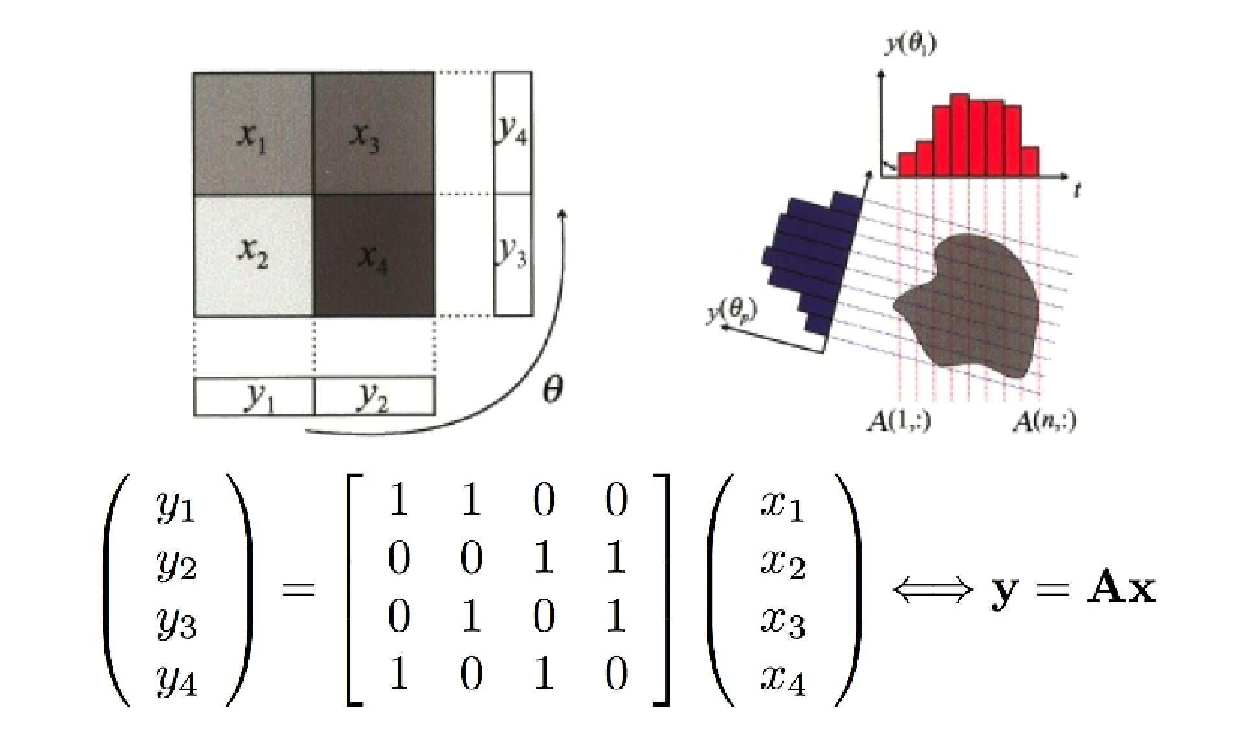
\includegraphics[width=0.7\linewidth]{tom_sketch.eps}}
\end{center}
\end{itemize}
}

\frame{
\titulo{Solar Rotational Tomography (SRT)}
\footnotesize
\vspace*{-0.25cm}
\begin{center}
{\bf
The object of study is the Solar Corona.\\
Solar rotation and telescope's orbit provide the multiple viewpoints.
}
\end{center}
\vspace{-1.cm}
\begin{columns}
%\vspace{-1cm}
\column{0.65\textwidth}
\ \ 
\vskip 0.5cm
\begin{itemize}
\item[\bu] 
\azul{Corona-K:} Thomson scatt. of photosph. \azul{WL} $\rightarrow$\\
diagnostic of coronal $\Ne$.
\item[\bu] \azul{SRT-WL} $\rightarrow$ 3D $\Ne$.
\item[\bu] {1st SRT-WL: Altschuler \& Perry (1972)}
\end{itemize}
\vskip 1cm
\begin{itemize}
\item[\bu] \azul{Corona-E:} coll-excited \azul{EUV} coronal emission $\rightarrow$\\
diagnostic of coronal $\Ne$ and $\Te$.
\item[\bu] \azul{SRT-EUV} $\rightarrow$ 3D EUV emissivity  $\rightarrow$\\
3D Differential Emission Measure $\rightarrow$\\
3D $\Ne$ y $\Te$.
\item[\bu] {1st SRT-EUV and \azul{DEM-Tomography}:\\ 
Vásquez, Frazin \& Kamalabadi (2009)\\
Frazin, Vásquez \& Kamalabadi (2009)}
\end{itemize}
\column{0.4\textwidth}
\vskip 1cm
\begin{center}
\azul{White Light Coronagraph}\\
\figu{\includegraphics[width=0.7\textwidth]{LASCOC2_comet.eps}}
\mediosalto
\azul{EUV Telescope}\\
\figu{\includegraphics[width=0.7\textwidth]{aia_211_fullsun.eps}}
\end{center}
\end{columns}
}

{
\setbeamercolor{normal text}{fg=white}
\setbeamercolor{frametitle}{fg=white}
\usebeamercolor[fg]{normal text}
\usebackgroundtemplate{\includegraphics[width=\paperwidth]{orbits_with_SDO.eps}}
\frame{
\titulo{Full-Sun WL and EUV Space Telescopes\\
       \vspace*{-.1cm}
        \hskip 3cm Circular Orbis with $R \approx 1$\,AU}
\footnotesize
\vspace{-2cm}
\begin{center}
Solar and Heliospheric Observatory {\bf(SOHO, 1996)}.
Sun-Earth L1 orbit.\\
Large Angle and Spectrometric Coronagraph {\bf (LASCO)}\\
Extreme ultraviolet Imaging Telescope {\bf (EIT)}.
\salto
Solar TErrestrial RElations Observatory {\bf(STEREO-A/B, 2007)}.
A/B Earth orbit.\\
White Light Coronagraphs {\bf (COR1 y COR2)}\\ 
Extreme UltraViolet Imager {\bf (EUVI)}.
\salto
Solar Dynamics Observatory {\bf(SDO, 2010)}.\\
Inclined geosynchronic orbit.\\
Atmospheric Imaging Assembly {\bf (AIA)}.
\salto
Ground-based Coronagraphs.
\end{center}
\vspace{-0.5cm}
}
}

%----------------------------------------------------------------------
\frame{
\titulo{SRT Computational Grid}
\vspace{-0.5cm}
\footnotesize
\begin{center}
\figu{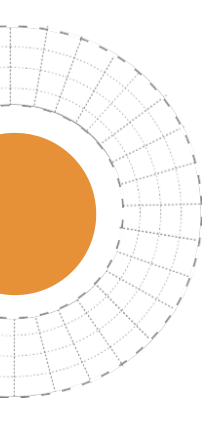
\includegraphics[width=0.25\textwidth,angle=90]{Grid.png}}
\\
Sun-centered spherical grid
\end{center}
\salto
\begin{columns}
\column{0.5\textwidth}
\centerline{\bf \underline{WL-SRT}}
\vskip 0.25cm
\begin{center}
FoV $\sim 2-8\,\Rs$\\ 
Cell $\sim 0.1\,\Rs \times 3\deg \times 3\deg$\\
\azul{\# Cells} $\azul{I}\,=\,60\times60\times120\sim\ \azul{4\times10^5}$\\
\azul{\# Pixels} $\azul{J}\,=\,512^2\times14\sim\ \azul{4\times10^6}$
\end{center}
\column{0.5\textwidth}
\centerline{\bf \underline{EUV-SRT}}
\vskip 0.25cm
\begin{center}
FoV $\sim 1-1.3\,\Rs$\\ 
Cell $\sim 0.01\,\Rs \times 2\deg \times 2\deg$\\
\azul{\# Cells} $\azul{I}\,=\,30\times90\times180\sim\ \azul{5\times10^5}$\\
\azul{\# Pixels} $\azul{J}\,=\,512^2\times14\times4\sim\ \azul{2\times10^7}$
\end{center}
\end{columns}
}

\frame{
\titulo{The SRT Problem}
\footnotesize

%-----------------------------------------------------------------------------
%\vspace{0.2cm}
%\begin{columns}
%\column{0.5\textwidth}
%\centerline{\bf \underline{WL-SRT}}
%\vskip 0.1cm
%FoV $\sim 2-8\,\Rs$.  Cell $\sim 0.1\,\Rs \times 3\deg \times 3\deg$\\
%\azul{\# Cells} $\azul{I}\,=\,60\times60\times120\sim\ \azul{4\times10^5}$\\
%\azul{\# Pixels} $\azul{J}\,=\,512^2\times14\sim\ \azul{4\times10^6}$
%\column{0.5\textwidth}
%\centerline{\bf \underline{EUV-SRT}}
%\vskip 0.1cm
%FoV $\sim 1-1.3\,\Rs$.  Cell $\sim 0.01\,\Rs \times 2\deg \times 2\deg$\\
%\azul{\# Cells} $\azul{I}\,=\,30\times90\times180\sim\ \azul{5\times10^5}$\\
%\azul{\# Pixels} $\azul{J}\,=\,512^2\times14\times4\sim\ \azul{2\times10^7}$
%\end{columns}
%\vspace{0.2cm}
%-----------------------------------------------------------------------------
\begin{center}
The signal recorded by the $j$-th pixel is given by:
\vskip 0.1cm
\figu{
$\azul{I_j} \ = \ \azul{ \int_{\textsf{LOS}_j} \ \textsf{d}l} \  
\azul{w(l)} \ \rojo{x(\azul{l})} 
\ \ \rightarrow \ \
\azul{\boldsymbol{I}} = \azul{\boldsymbol{A}\,\cdotp\,} \rojo{{\boldsymbol{X}}} $
}
\end{center}
\hskip 1.45cm
\azul{\ $\mathbf{I}$}: Vector of $\azul{J}$ elements $\azul{I_{j}}$, all pixels in all images.\\
\hskip 1.5cm
\azul{\,$\mathbf{A}$}: Large sparse matrix of $\azul{J\times I}$ elements $\azul{a_{j,i}}$, purelly geometrical.\\
\hskip 1.5cm
\rojo{\,$\rojo{\mathbf{X}}$}: Vector of $\azul{I}$ elements $\rojo{x_{i}}$, the discrete 3D distribution of the unknown:\\
\begin{center}
\begin{columns}
\column{0.5\textwidth}
\centerline{\bf \underline{WL-SRT}}
\vspace{-.5cm}
\begin{eqnarray*}
\rojo{x \left(\azul{{\bf r}}\right)} &=& 
\rojo{\Ne\left(\azul{{\bf r}}\right)}\\
\azul{w({\bf r})} &=& \azul{S_{\textsf{Thomson}}({\bf r})}
\end{eqnarray*}
\ \\
\column{0.5\textwidth}
\centerline{\bf \underline{EUV-SRT}}
\vspace{-.5cm}
\begin{eqnarray*}
\rojo{x \left(\azul{{\bf r}}\right)} &=&
\rojo{E_k\left(\azul{{\bf r}}\right)} \equiv \int_{0}^{\infty} \mathrm{d} \lambda \ \phi_k(\lambda)\ \eta (\mathbf{r}, \lambda)
\\
\azul{w({\bf r})} &=& \azul{1}
\end{eqnarray*}
\end{columns} 
\vskip 0.5cm
Solution: global optimization problem with cost function (of dimension-$I$):
\vskip 0.1cm
\figu{
$
f(\rojo{\boldsymbol{X}})
\ = \ 
\| \azul{\boldsymbol{I}} - \azul{\boldsymbol{A}}\cdotp\rojo{\boldsymbol{X}} \|^2
\ + \ 
p\ \|  \azul{\bR}\cdotp\rojo{\boldsymbol{X}}   \|^2
$
}
\\
\underline{1st term:} Difference between data and synthetic images.\\
\underline{2nd term:} Regularization of the solution.
\end{center}
}

\frame{
\titulo{Weighting Function for WL Thomson Scattering}
\footnotesize
\begin{center}
\figu{
$\azul{I_{\textsf{WL}}
\ = \
\int_{\textsf{LOS}} \, \textsf{d}l\ w(l)}\ \rojo{\Ne(l)}$
}
\salto
\begin{columns}
\column{0.5\textwidth}
\includegraphics[width=\textwidth,clip=]{LOS_sketch.png}
\column{0.5\textwidth}
\includegraphics[width=\textwidth,clip=]{WL_LOS_weighting.png}
\end{columns}
\salto
\figu{
$\azul{\mathbf{I}} = \azul{\bA\,\cdotp\,} \rojo{\Ne}$
\ \ $\rightarrow$ \ \ 
$f(\rojo{\Ne})
\ = \
\| \azul{\mathbf{I}} - \azul{\bA\,\cdotp\,} \rojo{\Ne} \|^2
\ + \
p\ \| \azul{\bR}\cdotp\rojo{\Ne} \|^2
$
}
\end{center}
}

\frame{
\titulo{SRT-WL Output: 3D Electron Density}
\scriptsize
\vspace{-0.25cm}
\begin{columns}
\column{0.5\textwidth}
\begin{center}
Ground-based coronagraph KCOR/HAO\\
FoV $\approx [1.1,2.5]\,\Rs$
\\
{\includegraphics[height=0.3\linewidth]{20171203_174921_kcor_image.jpg}}
{\includegraphics[height=0.3\linewidth]{20171217_181438_kcor_image.jpg}}
\\
CR-2198, Dec/17. Decline SC-24
\\
{\includegraphics[height=0.4\linewidth]{ne_kcor_map.png}}
\vskip 0.15cm
{\includegraphics[height=0.4\linewidth]{ne_kcor_rad_streamer.pdf}}
\\
\vspace{-0.1cm}
Lloveras et al. (2019)
\end{center}
\column{0.5\textwidth}
\begin{center}
Space-borne coronagraph LASCO-C2/SoHO\\
FoV $\approx [2.5,6.0]\,\Rs$
\\
{\includegraphics[height=0.3\linewidth]{20190626UT150155_23759824pB_image.jpg}}
{\includegraphics[height=0.3\linewidth]{20190703UT145410_23760695pB_image.jpg}}
\\
CR-2219, Jul/19 Eclipse Minim. SC-24/25
\\
{\includegraphics[height=0.4\linewidth]{ne_lascoc2_map.eps}}
\vskip 0.15cm
{\includegraphics[height=0.4\linewidth]{perfil_paper_necr2219_alto_simplepot.eps}}
\\
\vspace{-0.1cm}
Lloveras et al. (2022)
\end{center}
\end{columns}
}

\frame{
\titulo{SRT-EUV Output: 3D Filter Band Emissivity (FBE)}
\footnotesize
\vspace{-0.35cm}
\begin{columns}
\noindent
\column{0.075\textwidth}
\vskip 0.8cm
{\footnotesize
\hskip 0.05cm 171\,\AA
\vskip 1.75cm
\hskip 0.05cm 195\,\AA
\vskip 1.65cm
\hskip 0.05cm 284\,\AA
}
\column{\textwidth}
\begin{center}
{\footnotesize
{\bf \ \ \ Data Image\hfill $\rightarrow$ \hfill 3D FBE \hfill $\rightarrow$ \hfill Synthetic Image\ \ \ \ }
}\\
{\includegraphics[width=0.95\linewidth]{EUV_Tomography.png}}\\
\footnotesize
{\bf \ \ $\mathbf{1.03\,\Rs}$ \hskip 1cm $\mathbf{1.10\,\Rs}$ \hskip 1cm $\mathbf{1.15\,\Rs}$}
\end{center}
\end{columns}
\vskip 0.25cm
\centerline {Vásquez et al. (2009)}
}

\frame{
\titulo{EUV Narrowband Telescopes}
\footnotesize
\vspace{-0.4cm}
\begin{columns}
\column{0.5\textwidth}
\begin{center}
Signal at pixel $j$ of band $k$\\
$ I_{k,j}~[\textsf{ph/sec}] = \int \mathrm{d}\lambda  \ J_j(\lambda)  \ \azul{\phi_k(\lambda)} $\\
\vskip 0.1cm
\figu{\includegraphics[height=0.8\linewidth]{all_wave_a.eps}}
\\
Specific Intensity $J_j(\lambda)$\\
~[ph/\cmsq \,sr\,sec\,\AA]
\end{center}
\column{0.5\textwidth}
\begin{center}
\ \\
Each EUV bandpass \azul{$\phi_k$} selects Fe lines\\
emitted at different temperatures
\vskip 0.1cm
\figu{\includegraphics[height=0.75\linewidth]{euvi_bandpasses.eps}}
\\
\ \\
\ \\
\ 
\end{center}
\end{columns}
}

\frame{
\titulo{Detector Temperature Response: STEREO/EUVI}
\footnotesize
\vspace{-0.4cm}
$$
R_k(T) \ \ \equiv \ \ \int \mathrm{d} \lambda \ \ \phi_k(\lambda) \ \ {\eta( N_{e0}, \ba_0,
T; \lambda)} \ / \ {N_{e0}^2}
$$
\vspace{-0.5cm}
\begin{columns}
\column{0.25\textwidth}
\tr $\phi_k$: Bandpass $k$
\vskip 0.25cm
\tr $\eta(\lambda,T)$: \azul{\sc chianti}
\vskip 0.25cm
\tr Abundances:\\
Feldman et al. (1992)
\vskip 0.25cm
\tr Ionization eq.:\\ Bryans(2006)
\column{0.65\textwidth}
\begin{center}
\figu{\includegraphics[width=0.9\linewidth]{EUVI_Rk.eps}}
\\
Peak responses $\approx$ 1.0, 1.5, 2.0 MK.
\end{center}
\end{columns}
}

\frame{
\titulo{The Local Differential Emission Measure (LDEM)}
\footnotesize
\begin{itemize}
\item[\bu]
For each band \azul{$k$} we know now the FBE {$\azul{E_{k,i}}$} at each tomographic cell \azul{$i$}.
\salto
\item[\bu]
Using the temperature responses {$\azul{R_k(T)}$} the FBEs can be re-written as:
\vskip 0.1cm
\centerline{\figu{$\azul{E_{k,i} } \, = \, \azul{\int \mathrm{d}T \  R_k(T) \ \, \rojo{LDEM_i(T)} }$}}
\salto
\item[\bu]
The $\rojo{LDEM_i(T) \ [\textsf{cm}^{-6}\,\textsf{K}^{-1}]}$ of each cell \azul{$i$} is defined so that:
\begin{eqnarray*}
\langle \Ne^2 \rangle_i &=& {\hskip 0.8cm} \int \mathrm{d}T\ \rojo{LDEM_i(T)}\\
\langle \Te   \rangle_i &=& \frac{1}{\langle N_e^2\rangle_i } \int \mathrm{d}T\ \rojo{LDEM_i(T)}\ T\\
(W_T^2)_i &=&  \frac{1}{\langle N_e^2\rangle_i } \int \mathrm{d}T\ \rojo{LDEM_i(T)}\ \left(T-\langle \Te  \rangle_i\right)^2
\end{eqnarray*}
\end{itemize}
}

\frame{
\titulo{Finding the LDEM}
\footnotesize
\begin{columns}
\column{0.7\textwidth}
\begin{center}
A parametric model for the LDEM is chosen:
\vskip 0.1cm
\figu{$\rojo{LDEM_i(T)}=\mathcal{N}(T,\,\rojo{\mathbf{p}_i=[A,T_0,\sigma_T]_i})$,}
\\
and the following objective function is minimized:
\vskip 0.1cm
\figu{
$
g(\rojo{{\mathbf{p}}_i}) \ = \ 
\| \ \azul{ E_{k,i} }-
\azul{\int \mathrm{d}T \ \, R_k(T)\ \, \mathcal{N}(T,}\,\rojo{\mathbf{p}_i}\azul{)} \ 
\|^2 
$,
}
\\
to determine the LDEM in each cell.
\end{center}
\column{0.3\textwidth}
\begin{center}
\hspace{-1cm}
\frame{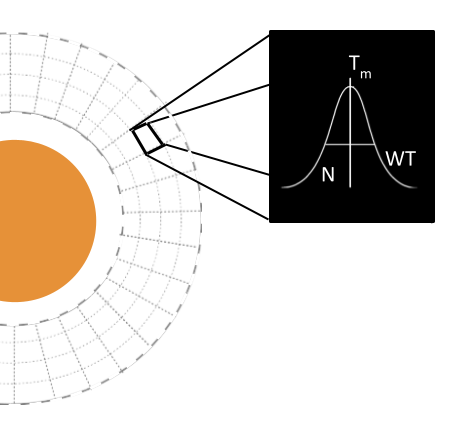
\includegraphics[height=\linewidth]{Grid_LDEM.png}}
\end{center}
\end{columns}
\begin{center}
\includegraphics[height=0.29\linewidth]{Densities.eps}
\hskip 0.2cm
\includegraphics[height=0.29\linewidth]{LDEMs.eps}
\\
Lat/Lon map of reconstructed $\Ne$ at a sample height, and LDEM at four cells. 
\end{center}
}

\frame{
\titulo{SRT-EUV + LDEM = DEM-Tomography (DEMT)}
\scriptsize
\vspace*{-0.25cm}
\begin{columns}
\column{0.35\textwidth}
\begin{center}
{\bf Band Emissivities}
\vskip 0.1cm
{\includegraphics[width=\linewidth]{FBE-EUVI-171.eps}}
\mediosalto
\ \\
{\includegraphics[width=\linewidth]{FBE-EUVI-195.eps}}
\mediosalto
\ \\
{\includegraphics[width=\linewidth]{FBE-EUVI-284.eps}}
\end{center}
\column{0.35\textwidth}
\begin{center}
{\bf Electron Density}
\\%\mediosalto
{\includegraphics[width=\linewidth]{Ne-2081-EUVI-l075.eps}}\\
\vskip 0.2cm
{\bf Electron Temperature}
\\%\mediosalto
{\includegraphics[width=\linewidth]{Tm-2081-EUVI-l075.eps}}\\
\vskip 0.2cm
$R=|1-E_{k,syn}/E_{k,tom}|$
\\%\mediosalto
{\includegraphics[width=\linewidth]{R-2081-EUVI-l075.eps}}
\end{center}
\end{columns}
}


\frame{
\titulo{Magnetograms and Coronal {\bf B} Extrapolations}
\footnotesize
\begin{columns}
\column{0.5\textwidth}
\figu{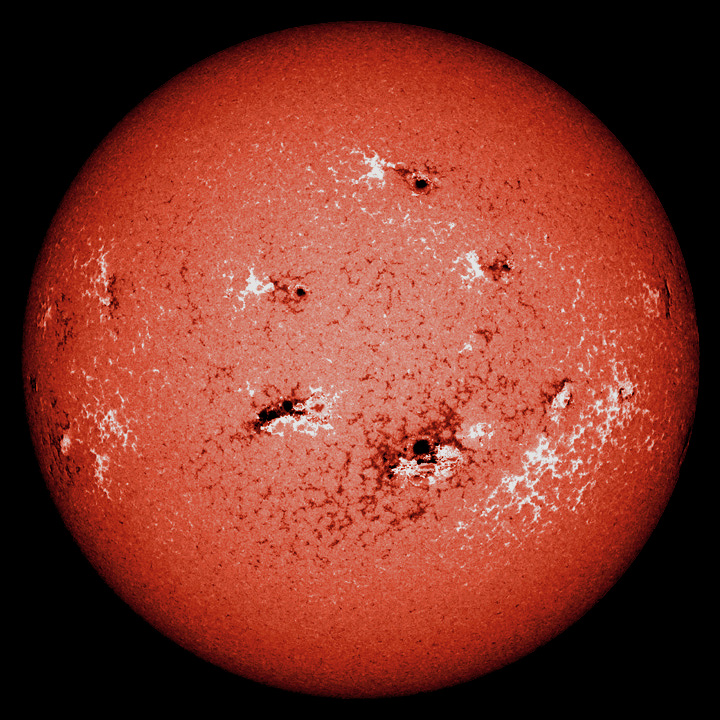
\includegraphics[width=0.9\textwidth]{magnetograma_esferico2.eps}}
\column{0.5\textwidth}
\figu{\includegraphics[width=0.9\textwidth]{CR2081-PFSS.eps}}
\end{columns}
\begin{columns}
\column{0.2\textwidth}
\column{0.3\textwidth}
$\nabla \cdot B = \nabla \cdot (\nabla \Phi)  = 0$
\column{0.3\textwidth}
\begin{equation*}
\left\lbrace
  \begin{array}{l}
%\begin{align}
 %\nabla \cdot B = \nabla \cdot (\nabla \Phi) & = 0 \nonumber \\
 \frac{\partial \Phi}{\partial r} (r=1\mrsun,\theta,\phi)  = M(\theta,\phi) \nonumber \\
 \ \nonumber \\
 \Phi(r=R,\theta,\phi)  = 0 \nonumber
%\end{align}
\end{array}
\right.
\end{equation*}
\column{0.2\textwidth}
\end{columns}
}

\frame{
\titulo{Tomography and {\bf B}-Models}
\begin{columns}
\column{0.5\textwidth}
\begin{center}
\includegraphics[height=0.5\linewidth]{eclipse_2008.eps}
\includegraphics[width=0.8\linewidth]{Ne_1.035_cr2077-euviB_l1.0.eps}
\includegraphics[width=0.8\linewidth]{Ne_1.075_euvi-b_cr2077.eps}
\end{center}
\column{0.5\textwidth}
\begin{center}
\includegraphics[height=0.5\linewidth]{CR-2081-FDIPS.eps}
\includegraphics[width=0.8\linewidth]{Tm_1.035_cr2077-euviB_l1.0.eps}
\includegraphics[width=0.8\linewidth]{Tm_1.075_euvi-b_cr2077.eps}
\end{center}
\end{columns}
}

\frame{
\titulo{Tomographic Results along {\bf B}-lines}
\footnotesize
\begin{center}
\figu{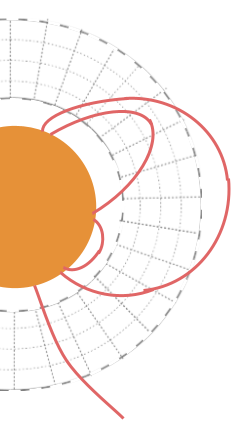
\includegraphics[height=0.35\linewidth]{Grid-loops.png}}
\figu{\includegraphics[height=0.35\linewidth]{Traced-Loop.eps}}
\salto
DEMT results along individual {\bf B}-lines are characterized by parametric fits:
\begin{eqnarray*}
\Ne(h) &=& N_0\ \textsf{exp}\left(-h/\lambda\right)
\\
\Te(h) &=& T_0 \, + \, \gamma \, h
\end{eqnarray*}
and fitting parameters are analyzed statistically.
\end{center}
}

\frame{ 
\titulo{Space Weather Modeling Framework}
\begin{columns}
\column{0.5\textwidth}
\figu{\includegraphics[width=\textwidth]{oran_swmf_2015.png}}
\column{0.4\textwidth}
\footnotesize
\bu CLASP / U. of Michigan
\vskip 0.10cm
\hskip 0.25cm (Toth et al., 2012)
\vskip 0.5cm
\bu Sun -- Heliosphere -- IM\\
\vskip 0.5cm
\bu Multiple modules\\
\vskip 0.5cm
\bu Solar Corona Solar Wind module:
\vskip 0.3cm
\hskip 0.3cm
\figu{3D-MHD \azul{\sc a.w.so.m.}}
\vskip 0.10cm
\hskip 0.25cm (van der Holst et al., 2014)
\end{columns}
}

\frame{
\titulo{DEMT Validation of {\sc awsom}: Coronal Base}
\footnotesize
\begin{columns}
\column{0.7\textwidth}
\begin{center}
\includegraphics[width=0.49\textwidth,clip=]{map_Ne_CR2219_DEMT-AIA_H1_L834_r3d_multistart_1105_Rsun2219.eps}
\includegraphics[width=0.49\textwidth,clip=]{map_Tm_CR2219_DEMT-AIA_H1_L834_r3d_multistart_1105_Rsun2219_2.eps}
\vskip 0.25cm
\includegraphics[width=0.49\textwidth,clip=]{map_Ne_awsom_2219_ener_new_1105_Rsun2219.eps}
\includegraphics[width=0.49\textwidth,clip=]{map_Te_awsom_2219_ener_new_1105_Rsun2219_2.eps}
\vskip 0.25cm
\includegraphics[width=0.49\textwidth,clip=]{perfil_paper_necr2219_bajo.eps}
\includegraphics[width=0.49\textwidth,clip=]{perfil_paper_tecr2219_bajo.eps}
\\
\vspace{-0.05cm}
Lloveras et al. (2022)
\end{center}
\column{0.3\textwidth}
\bu Analysis of campaigns of Whole Heliosphere and Planetary Interactions (WHPI).
\vskip 0.5cm
\bu Consistent North O/C and CH.
\vskip 0.5cm
\bu Southern O/C shifted $\approx +20^\circ$ from CH.
\vskip 1.5cm
\bu $\Delta\Ne(r) \approx \pm 5\%$.
\vskip 0.5cm
\bu $\Delta\Te(r) \approx -15\%$.
\vskip 0.5cm
Lloveras et al. (2022)
\end{columns}
}

\frame{
\titulo{EUV Synthetic Images: SRT vs. {\sc awsom}}
\footnotesize
\begin{center}
\includegraphics[width=\textwidth,clip=]{Figura_2_paper_imag_sinteticas_2.eps}
\salto
{\sc awsom} O/C discrepancy due to lack of accuracy of boundary condition. 
\vskip 0.5cm
Lloveras et al. (2022)
\end{center}
}

\frame{
\titulo{WL-SRT Validation of {\sc awsom}: Larger Heights}
\footnotesize
\begin{center}
\includegraphics[width=0.35\textwidth,clip=]{map_LASCOC2pB_CR2223_24hr-Cadence_Rmin225_Rmax825_IRmin25_IRmax60_60x60x120_BF2_r3D_l25e-5_vfinal_interpolado_2500_Rsun2223.eps}
\includegraphics[width=0.35\textwidth,clip=]{map_Ne_awsom_2223_ener_new_2505_Rsun2219.eps}
\includegraphics[width=0.28\textwidth,clip=]{perfil_paper_necr2223_alto_simplepot.eps}
\\
$\Delta\Ne$ up to $+75\%$ at these larger heights $\rightarrow$ model's acceleration rates are too low.\\ 
Current efforts include improvement in the energy cascading process of model.
\vskip 1cm
\includegraphics[width=\textwidth,clip=]{Figura_7_paper_imag_sintetica_2.eps}
\vskip 0.75cm
Lloveras et al. (2022)
\end{center}
}

\frame{
\titulo{DEMT Validation of 3D Solar Wind Model}
\footnotesize
\begin{center}
\includegraphics[width=0.45\textwidth,clip=]{map_Vr_awsom_2223_realization10_extended_new_5995_Rsunsom_.jpg}
\includegraphics[width=0.45\textwidth,clip=]{scatter_plot_Vr_newtrace_20_CR-2223_filtro.eps}
\\
\includegraphics[width=0.45\textwidth,clip=]{scatter_plot_nedemtFIT_1055_vs_vrxsignoBr_20rs_CR-2223_trace_chip_.eps}
\includegraphics[width=0.45\textwidth,clip=]{scatter_plot_tmdemt_MEAN_vs_vrxsignoBr_20rs_CR-2223_Test_trace_chip_.eps}
Lloveras et al. (2022)
\end{center}
\bu Model's terminal wind speed anticorrelates with DEMT $\Ne$ and $\Te$ at source region.
\vskip 0.1cm
\bu Consistent with stable highly ionized slow wind flowing around Streamers $\rightarrow$\\
\hskip 0.3cm
No reconection process required (Oran et al., 2015).
}

\frame{
\titulo{The Solar Cycle and Coronal Activity}
\footnotesize
\begin{columns}
\column{0.5\textwidth}
\begin{center}
Babcock et al. (1961)\\
\includegraphics[width=0.7\textwidth]{babckok_model.png}
\end{center}
\column{0.5\textwidth}
\bu Solar dynamo $\rightarrow$ $\mathbf{B}(t)$.\\
\vskip 0.4cm
\bu Minima: Global dipole, few SSs/ARs.\\
\vskip 0.4cm
\bu Maxima: Multipole, many SSs/ARs.\\
\vskip 0.4cm
\bu Period $\approx 11$ years.\\
\end{columns}
\begin{center}
\includegraphics[width=0.99\textwidth]{SC_22-25.pdf}
\\
Space Weather Prediction Center (NOAA)
\end{center}
}

\frame{
\titulo{Rotations Selected from each Minima}
\vspace{-0.5cm}
\begin{center}
\includegraphics[width=0.8\textwidth]{ciclos_ssn_recorte3.pdf}
\end{center}
}

\frame{
\titulo{DEMT Comparative Solar Minima Study}
\footnotesize
\vspace{-0.25cm}
\begin{center}
\figu{\includegraphics[width=0.99\textwidth]{DEMT.png}}
\end{center}
\bu Global thermodynamic state of minima not correlated with activity level of full cycle.
\vskip 0.1cm
\bu $\Te$ correlates with the minima activity intermitency level.
\vskip 0.1cm
\bu Loops with ${\d}T/{\d}r<0$ systematically found in the Streamer core of all minima $\rightarrow$\\
\hskip 0.25cm
reproduced by Alfvén wave heating models (Shiff \& Cranmer, 2016).
}

\frame{
\titulo{DEMT and the Coronal Heating problem}
\footnotesize
\begin{center}
\figu{\includegraphics[width=0.95\textwidth]{balance.png}}
\end{center}
}

\frame{
\titulo{DEMT Energy Flux}
\footnotesize
\begin{center}
\figu{\includegraphics[width=0.65\textwidth]{Flujos.png}}
\\
$\Phi_{\textsf{h}}$ Consistent with coronal base Alfvén wave energy flux
$1.5-2.5~\erg\,\cm^{-2}\,\sec^{-1}$\\
from spectroscopic data (Hahn \& Savin, 2014).
\\
Lloveras et al. (2020)
\vskip 0.2cm
Current project: coronal heating rate.
\end{center}
}

\frame{
\titulo{Parker Solar Probe (PSP)}
{\footnotesize\sf
\begin{center}
Launched 12 August 2018.\\
Nearly ecliptic-plane extremely eccentric orbits.\\ 
Decreasing perihelion $\approx 13-10~\mrsun$ in 2022-2025.
\salto
\figu{
{\includegraphics[height=0.49\textwidth]{PSP_XY-Plane.png}}
{\includegraphics[height=0.49\textwidth]{PSP_Ecliptic-EdgeOn.png}}
}
\end{center}
}}

\frame{
\titulo{PSP/WISPR Telescope}
{\footnotesize\sf
\begin{center}
Intrumentation includes the wide-angle WISPR\\ 
WL telescopes, with off-West-limb square FoVs.
\salto
\figu{\includegraphics[height=0.5\textwidth]{wispr_FOV.png}}
\end{center}
}}

\frame{
\titulo{PSP/WISPR Synthetic WL Images}
{\footnotesize\sf
\begin{center}
\includegraphics[width=0.3\textwidth,clip=]{comp_x_AWSOM_CR2082_WISPR_I_2018-11-01T071114.eps}
\includegraphics[width=0.3\textwidth,clip=]{comp_x_AWSOM_CR2082_WISPR_I_2018-11-06T183729.eps}
\\
Solar minimum simulation -- Orbit 01 (2018-Nov, Perihelion 0.17~AU)
\\
\hrulefill
\\
\includegraphics[width=0.3\textwidth,clip=]{comp_x_AWSOM_CR2082_WISPR_I_2025-06-14T165408.eps}
\includegraphics[width=0.3\textwidth,clip=]{comp_x_AWSOM_CR2082_WISPR_I_2025-06-19T124225.eps}
\\
Solar minimum simulation -- Orbit 24 (2025-Jun, Perihelion 0.05~AU)
\end{center}
}}

\frame{
\titulo{Simulations of SRT-WL with PSP/WISPR}
{\footnotesize\sf
\begin{center}
PSP close proximity to the Sun during 2022-2025 implies very-fast orbital speed.\\ 
Data required for tomography will be gathered in $< 3$~days.\\ 
Fastest reconstructions to-date, minimizing dynamics-induced artifacts.
\salto
\figu{\includegraphics[width=0.7\textwidth]{wispr_tom.png}}
\\
Vásquez et al. (2019)
\salto
Simulations show that about half the solar corona longitudes can be tomographically reconstructed with data taken between 2022 (left) and 2025 (right).
\end{center}
}
}

\frame{
\titulo{Solar Orbiter (SOLO)}
{\footnotesize\sf
\begin{center}
Launched 10 February 2020.\\
Highly eccentric orbits with increasing off-ecliptic\\ 
inclination $\approx 0-33^\circ$ in 2022-2029.
\salto
\figu{
{\includegraphics[height=0.49\textwidth]{SOLO_XY-Plane.png}}
{\includegraphics[height=0.49\textwidth]{SOLO_Ecliptic-EdgeOn.png}}
}
\end{center}
}}

\frame{
\titulo{SOLO/Metis Coronagraph}
{\footnotesize\sf
\begin{center}
Intrumentation includes the Metis\\
WL and Ly-$\alpha$ coronagraph.
\salto
\figu{
{\includegraphics[height=0.49\textwidth]{metis_fov_1.jpg}}
{\includegraphics[height=0.49\textwidth]{metis_fov_2.jpg}}
}
\end{center}
}}

\frame{
\titulo{SOLO Orbit}
{\footnotesize\sf
\begin{center}
\figu{\includegraphics[width=0.9\textwidth,clip=]{plot_with_gam.eps}}
\end{center}
}
}

\frame{
\titulo{SOLO/Metis Synthetic WL Images}
\footnotesize
\begin{center}
\includegraphics[width=0.3\textwidth,clip=]{Fig_Aphelion_CR2152_serie_a_colorBAR.jpg}
\\
\includegraphics[width=0.22\textwidth,clip=]{Fig_Aphelion_CR2152_serie_a.jpg}
\includegraphics[width=0.22\textwidth,clip=]{Fig_Aphelion_CR2152_serie_b.jpg}
\includegraphics[width=0.22\textwidth,clip=]{Fig_Aphelion_CR2152_serie_c.jpg}
\\
SolMax simulation - Aphelion observation (2023-Jan, $D \approx 0.94$~AU)
\\
\hrulefill
\\
\includegraphics[width=0.3\textwidth,clip=]{Fig_Perihelion_CR2152_serie_a_colorBAR.jpg}\\
\includegraphics[width=0.22\textwidth,clip=]{Fig_Perihelion_CR2152_serie_a.jpg}
\includegraphics[width=0.22\textwidth,clip=]{Fig_Perihelion_CR2152_serie_b.jpg}
\includegraphics[width=0.22\textwidth,clip=]{Fig_Perihelion_CR2152_serie_c.jpg}
\\
SolMax simulation - Perihelion observation (2023-Mar, $D \approx 0.4-0.3-0.4$~AU)
\end{center}
}

\frame{
\titulo{Simulations of SRT-WL with SOLO/Metis}
{\footnotesize\sf
\vspace{-0.1cm}
\begin{center}
\hskip 1.5cm Aphelion \hfill Perihelion \hfill Maximum Latitude \ \ \ \ \ \ \ \ \
\\
\includegraphics[width=0.3\textwidth,clip=]{Fig_Ne_AWSOM-CR2152_interp_aphelion_10_20_Rsun.jpg}
\includegraphics[width=0.3\textwidth,clip=]{Fig_Ne_AWSOM-CR2152_interp_perihelion_dlon06DEG_3_150_Rsun.jpg}
\includegraphics[width=0.3\textwidth,clip=]{Fig_Ne_AWSOM-CR2152_interp_maxlat_4_950_Rsun.jpg}
\vspace{-0.2cm}
\includegraphics[width=0.3\textwidth,clip=]{Fig_Ne_Metis_CR2152_aphelion_dlon06DEG_10_20_Rsun.jpg}
\includegraphics[width=0.3\textwidth,clip=]{Fig_Ne_Metis_CR2152_perihelion_dlon06DEG_3_150_Rsun.jpg}
\includegraphics[width=0.3\textwidth,clip=]{Fig_Ne_Metis_CR2152_maxlat_dlon06DEG_4_950_Rsun.jpg}
\\
\includegraphics[width=0.3\textwidth,clip=]{Fig_ratio_Ne_CR2152_aphelion_dlon06DEG_10_20_Rsun.jpg}
\includegraphics[width=0.3\textwidth,clip=]{Fig_ratio_Ne_CR2152_perihelion_dlon06DEG_3_150_Rsun.jpg}
\includegraphics[width=0.3\textwidth,clip=]{Fig_ratio_Ne_CR2152_maxlat_dlon06DEG_4_950_Rsun.jpg}
\\
\includegraphics[width=0.3\textwidth,clip=]{cr2152_dlon06_aphelion_awsom_tom_ratio_5_700-10_30_Rsun.eps}
\includegraphics[width=0.3\textwidth,clip=]{comp_cr2152_perih_dlon06_awsom_vs_tom_range2_400-3_200_Rsun.eps}
\includegraphics[width=0.3\textwidth,clip=]{comp_cr2152_maxlat_6deg_awsom_tom_rat_range3_500-5_000_Rsun.eps}
\vspace{0.05cm}
Vásquez, Nuevo, et al. (2022)
\end{center}
}
}

\frame{
\titulo{3D Solar Wind Speed from WL+Ly$\alpha$ Tomography}
\footnotesize
\begin{center}
SOLO/Metis also takes Ly$\alpha$ images.
\vskip 0.2cm
Coronal Ly$\alpha$ emitted by neutral H \azul{radiativelly excited} by the photospheric emission:
\vskip 0.2cm
\figu{
$
\azul{I_{\textsf{Ly$\alpha$}}} \ = \ \azul{ \int_{\textsf{LOS}} \ \textsf{d}l} \  
\azul{\Gamma(l)} \ \rojo{\DH(\azul{l})} 
\ \ \rightarrow \ \
\azul{\boldsymbol{I}} = \azul{\boldsymbol{A}\,\cdotp\,} \rojo{\DH}
$
}
\vskip 0.05cm
where the geometrical dilution factor $\azul{\Gamma(r)}$ is known and:
\vskip 0.2cm
\figu{
$
\rojo{\DH} \equiv \rojo{\NH \ D}, 
\ \ \textsf{``Doppler dimming" term:} \ \
\rojo{D} \equiv \int\dnu\ I_\odot(\nu + \delta\nu)\ \phi(\nu-\nu_0)
$
}
\vskip 0.2cm
\figu{
$
\rojo{\NH} \approx 0.8\ \RH(\Te)\ \rojo{\Ne}
\ \rightarrow \ \
\rojo{D} = (1 /0.8\ \RH(\Te)) \ \rojo{\DH/\Ne} 
$
}
\vskip 0.2cm
$\rojo{\DH}$ and $\rojo{\Ne}$ are respectivelly obtained from Ly$\alpha$ and WL tomography.\\
\salto
The reconstructed $\rojo{D}$ can be related to the solar wind velocity and $\TH$ as:
\vskip 0.2cm
\figu{
$
D(v_r) = 
I_0 \ \lambda_0\
\frac{1}{\sqrt{{\sigma_{\textsf{disk}}^2+\sigma_{\textsf{cor}}^2}}}\
\textsf{exp}\left[-\frac{v_r^2}{({\sigma_{\textsf{disk}}^2+\sigma_{\textsf{cor}}^2})}\right]
$
}
\vskip 0.2cm
\figu{
$
\sigma_{\textsf{cor}} = \sqrt{(\textsf{cos}\beta\,\Vthpar)^2+(\textsf{sin}\beta\,\Vthper)^2}
\ \ \textsf{and} \ \ 
\beta\equiv\textsf{cos}^{-1}(B_r/B)
$
}
\end{center}
}

\frame{
\titulo{SOLO/Metis Synthetic WL and Lyman-$\alpha$ Images}
\footnotesize
\begin{center}
\includegraphics[width=0.3\textwidth,clip=]{Fig_Perihelion_serie_a_colorBAR.jpg}\\
\includegraphics[width=0.22\textwidth,clip=]{Fig_Perihelion_serie_a.jpg}
\includegraphics[width=0.22\textwidth,clip=]{Fig_Perihelion_serie_b.jpg}
\includegraphics[width=0.22\textwidth,clip=]{Fig_Perihelion_serie_c.jpg}
\\
\azul{WL:} SolMin simulation - Perihelion observation (2023-Mar, $D \approx 0.4-0.3-0.4$~AU)
\\
\hrulefill
\\
\includegraphics[width=0.3\textwidth,clip=]{Fig_Perihelion_lya_serie_a_colorBAR.jpg}\\
\includegraphics[width=0.22\textwidth,clip=]{Fig_Perihelion_lya_serie_a.jpg}
\includegraphics[width=0.22\textwidth,clip=]{Fig_Perihelion_lya_serie_b.jpg}
\includegraphics[width=0.22\textwidth,clip=]{Fig_Perihelion_lya_serie_c.jpg}
\\
\azul{L$\alpha$:} SolMin simulation - Perihelion observation (2023-Mar, $D \approx 0.4-0.3-0.4$~AU)
\end{center}
}

\frame{
\titulo{Simulations of SRT-Ly$\alpha$ with SOLO/Metis}
\footnotesize
\begin{center}
\includegraphics[width=0.49\textwidth]{DH_Vr_half_AWSOM_perihelionB_2_450_Rsun.jpg}
\includegraphics[width=0.49\textwidth]{DH_Vr_half_TOM_perihelionB_2_450_Rsun.jpg}
\\
\includegraphics[width=0.49\textwidth]{DH_Vr_half_RATIO_perihelionB_2_450_Rsun.jpg}
\includegraphics[width=0.49\textwidth]{comparison_DH_vr_half_PerihelionB_ratio_range2_400-3_200_Rsun.eps}
\salto
\ \ \\
\ \ 
\end{center}
}

\frame{
\titulo{Reconstruction of Wind Speed}
\footnotesize
\begin{center}
\includegraphics[width=0.49\textwidth]{Vr_Vr_half_AWSOM_perihelionB_2_450_Rsun.jpg}
\includegraphics[width=0.49\textwidth]{Vr_Vr_half_TOM_perihelionB_2_450_Rsun.jpg}
\\
\includegraphics[width=0.49\textwidth]{Vr_Vr_half_RATIO_perihelionB_2_450_Rsun.jpg}
\includegraphics[width=0.49\textwidth]{comparison_Vr_vr_half_PerihelionB_ratio_range2_400-3_200_Rsun.eps}
\salto
Nuevo, Vásquez, Metis-team \& Michigan\\ 
(under development)
\end{center}
}

\frame{
\titulo{Current and Future Projects}
\footnotesize
\begin{itemize}

\item[\bu] SDO/AIA and STEREO/EUVI DEMT analysis of:\\
+ Temperature structure evolution along SC 24/25 minimum phase.\\
+ Coronal heating rate maps.

\salto

\item[\bu] SRT with actual data of PSP/WISPR and SolO/Metis.

\salto

\item[\bu]
\azul{Multi-Instrument Tomography (MIT)}\\
Vásquez, Nuevo \& Michigan:\\
+ \azul{SDO/AIA}  $\rightarrow$ 3D filter band emissivity in $1-3~$MK bands.\\
+ \azul{HAO/KCor} $\rightarrow$ 3D $\Ne$.\\
+ \azul{HAO/UCoMP} (Upgraded Coronal Multichannel Polarimeter, \azul{2022}):\\
\hskip 2.5cm Several $1-3$~MK coronal visible Fe lines $\rightarrow$ 3D emissivity.\\
- Common FoV $\approx 1.1-1.3~\Rs$.\\
- Joint analysis of all SRT products $\rightarrow$ \azul{3D $\Ne$, $\Te$, $W_N$, $W_T$ and [Fe]}.

\salto

\item[\bu]
\azul{Validation of CME Simulations}\\ 
Diego Lloveras et al. (Mendoza--IAFE--Michigan):\\
+ {SWMF} CME simulations involve two modules: \azul{\sc awsom} and \azul{\sc eeg}.\\
+ DEMT and WL-SRT to validate \azul{\sc awsom}.\\
+ CME observations (H$\alpha$, EUV-304\AA, magnetograms and WL) to validate \azul{\sc eeg}.

\end{itemize}

}

\end{document}
